\documentclass{article}\usepackage[]{graphicx}\usepackage[]{color}
%% maxwidth is the original width if it is less than linewidth
%% otherwise use linewidth (to make sure the graphics do not exceed the margin)
\makeatletter
\def\maxwidth{ %
  \ifdim\Gin@nat@width>\linewidth
    \linewidth
  \else
    \Gin@nat@width
  \fi
}
\makeatother

\definecolor{fgcolor}{rgb}{0.345, 0.345, 0.345}
\newcommand{\hlnum}[1]{\textcolor[rgb]{0.686,0.059,0.569}{#1}}%
\newcommand{\hlstr}[1]{\textcolor[rgb]{0.192,0.494,0.8}{#1}}%
\newcommand{\hlcom}[1]{\textcolor[rgb]{0.678,0.584,0.686}{\textit{#1}}}%
\newcommand{\hlopt}[1]{\textcolor[rgb]{0,0,0}{#1}}%
\newcommand{\hlstd}[1]{\textcolor[rgb]{0.345,0.345,0.345}{#1}}%
\newcommand{\hlkwa}[1]{\textcolor[rgb]{0.161,0.373,0.58}{\textbf{#1}}}%
\newcommand{\hlkwb}[1]{\textcolor[rgb]{0.69,0.353,0.396}{#1}}%
\newcommand{\hlkwc}[1]{\textcolor[rgb]{0.333,0.667,0.333}{#1}}%
\newcommand{\hlkwd}[1]{\textcolor[rgb]{0.737,0.353,0.396}{\textbf{#1}}}%
\let\hlipl\hlkwb

\usepackage{framed}
\makeatletter
\newenvironment{kframe}{%
 \def\at@end@of@kframe{}%
 \ifinner\ifhmode%
  \def\at@end@of@kframe{\end{minipage}}%
  \begin{minipage}{\columnwidth}%
 \fi\fi%
 \def\FrameCommand##1{\hskip\@totalleftmargin \hskip-\fboxsep
 \colorbox{shadecolor}{##1}\hskip-\fboxsep
     % There is no \\@totalrightmargin, so:
     \hskip-\linewidth \hskip-\@totalleftmargin \hskip\columnwidth}%
 \MakeFramed {\advance\hsize-\width
   \@totalleftmargin\z@ \linewidth\hsize
   \@setminipage}}%
 {\par\unskip\endMakeFramed%
 \at@end@of@kframe}
\makeatother

\definecolor{shadecolor}{rgb}{.97, .97, .97}
\definecolor{messagecolor}{rgb}{0, 0, 0}
\definecolor{warningcolor}{rgb}{1, 0, 1}
\definecolor{errorcolor}{rgb}{1, 0, 0}
\newenvironment{knitrout}{}{} % an empty environment to be redefined in TeX

\usepackage{alltt}
\usepackage[sc]{mathpazo}
\usepackage[T1]{fontenc}
\usepackage{geometry}
\geometry{verbose,tmargin=2.5cm,bmargin=2.5cm,lmargin=2.5cm,rmargin=2.5cm}
\setcounter{secnumdepth}{2}
\setcounter{tocdepth}{2}
\usepackage{url}
\usepackage[unicode=true,pdfusetitle,
 bookmarks=true,bookmarksnumbered=true,bookmarksopen=true,bookmarksopenlevel=2,
 breaklinks=false,pdfborder={0 0 1},backref=false,colorlinks=false]
 {hyperref}
\hypersetup{
 pdfstartview={XYZ null null 1}}
\usepackage{breakurl}
\title{Simple Regression Analysis}

\author{Joelle Shane}

\date{\today}
\IfFileExists{upquote.sty}{\usepackage{upquote}}{}
\begin{document}
\maketitle

\begin{abstract}
Reproducability in science is an increasingly important concept. In order to verify results and build off of them, we must be able to reproduce work. This report attempts to reproduce results shown in chapter 3.1 of the book An Introduction to Statistical Learning. The same data is used (and can be downloaded at http://www-bcf.usc.edu/~gareth/ISL/Advertising.csv) and a simple regression is run to see if are results match the original results. 
\end{abstract}

\section{Introduction}

Advertising can be extremely costly, but also extremely effective. The goal is to spend as little on advertising as possible while seeing the most payoff as an increase in sales. By running a simple linear regression, we can estimate the effect advertising has on sales and therefore extrapolate that to how worthwhile a method of advertising is. If we know the expected increase of sales for every increase of TV advertising, we can then calculate how much money we are spending on advertising verus how much money we make from the addionional sales and see if the method of avertising is profitable. If it's profitable, we can increase expenditure in that avenue to increase sales but we also might see expenditures in different areas of advertisment bring even more sales and more returns. The scope of this report just focuses on the effect TV advertising has on sales but it is important to understand the broad application regression such as this one can have in a business setting. 

\section{Data}

The data used for this report is advertising data of a product that includes the sales (measured in thousands of units) of a product across two hundred different markets and the amount spend on advertising (measured in thousands of dollars). The advertising data is colleced in three different avenues of advertising: television, radio, and newspaper. Each entry in the data set has the corresponding amount spent on the different advertising media and the corresponding amount of sales of the product in that time period. 

\section{Methodology}

To analyze the effect of advertising by television on the amount of sales, a simple linear regression is run. This method holds the amount of advertising on radio and newspapers constant and only varies the amount of advertising spend on television, then measures the change in sales corresponding to a one unit change in the amount of money spent on telvision advertisment. This gives us an estimate of the effect television advertising has on total sales. The model for this regression is as follows:

Simple Linear Regression : $Y = B_0 + X_1B_1 + u$

\begin{itemize}

\item $Y$ : Total Sales

This is the dependent variable in our model and is effected by the amount of money spent on TV advertising. We calculate this predicted value based on the other elements of the model.

\item $B_0$ : Intercept

The intercept is the amount of sales of the produce we would see even with no money spent on television advertising. Of course, it is natural to assume that we would sell some amount of product without any advertising at all.

\item $B_1$ : Coefficient on TV advertising

The coefficinet on TV advertising represents the amount we predict to see total sales increase if we increase the amount spent on TV advertising by one unit. This follows from assuming advertising has an effect on sales and calculating what that effect is from the data set. 

\item $X_1$ : TV advertising amount 

This is the independent variable in the model. Given the chosen amount of TV advertising, we can calculate the expected value of total sales. 

\item $u$ : error

The error term is random noise and something for which we cannot control. This incorporates the idea that while we predict sales will be one thing, it might not hit that exact target due to random chance. 
\end{itemize}

\section{Results}

\begin{knitrout}
\definecolor{shadecolor}{rgb}{0.969, 0.969, 0.969}\color{fgcolor}\begin{kframe}
\begin{alltt}
\hlkwd{load}\hlstd{(}\hlstr{"../../stat159-hw02/data/regression.RData"}\hlstd{)}
\hlstd{a}
\end{alltt}
\begin{verbatim}
## 
## Call:
## lm(formula = Sales ~ TV, data = advertising)
## 
## Residuals:
##     Min      1Q  Median      3Q     Max 
## -8.3860 -1.9545 -0.1913  2.0671  7.2124 
## 
## Coefficients:
##             Estimate Std. Error t value Pr(>|t|)    
## (Intercept) 7.032594   0.457843   15.36   <2e-16 ***
## TV          0.047537   0.002691   17.67   <2e-16 ***
## ---
## Signif. codes:  0 '***' 0.001 '**' 0.01 '*' 0.05 '.' 0.1 ' ' 1
## 
## Residual standard error: 3.259 on 198 degrees of freedom
## Multiple R-squared:  0.6119,	Adjusted R-squared:  0.6099 
## F-statistic: 312.1 on 1 and 198 DF,  p-value: < 2.2e-16
\end{verbatim}
\end{kframe}
\end{knitrout}

From the summary statistics we can see that TV advertising has an estimated coefficen tof 0.048. This means that for every one thousand dollar increase in TV spending, there is an increase in total sales by 48. We also get the standard error assosiated with that value which allows us to calculate the t statistic and p-value. The p-value is almost zero and is definitely under the threshold (0.05) to conclude that this result was not obtained by chance and in fact TV advertising has a real effect on sales. 

The R-squared value tells us how much of the chance in Y is explained by the change in X. Here our R-squared value is about 0.6 which means that around 60\% of the change in total sales is due to the change in expenditure in TV advertising. This is a strong R-squared value and we can conclude that the data is explained well by our model. 

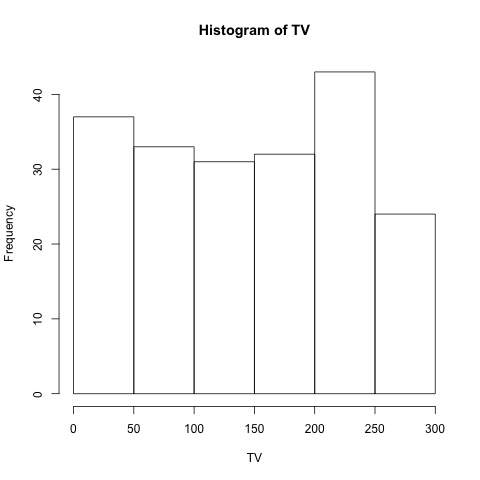
\includegraphics[height=2in]{../../stat159-hw02/images/histogram-tv.png}
 
\centerline{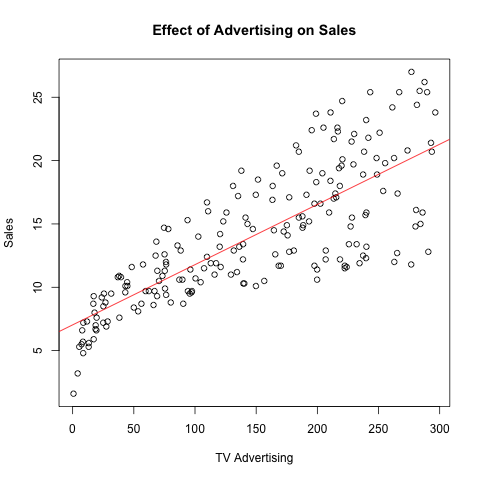
\includegraphics[height=2in]{../../stat159-hw02/images/scatterplot-tv-sales.png}}
 
We can see the visual realization of the regression in this plot. There is a positive correlation between TV advertising and sales, hence the positive slope of the graph. The best fit line (in red) shows us our prediction of where total sales should be given TV advertising, based on our estimate of the coefficient from the data. The slope of this line is equal to the coefficient and is equal to 0.048. If all the dots were perfectly on the line, this would mean every outcome matched every prediction the model made, and there would be no random chance. Where deviations from the line occur, we explain this as random error that we cannot control. 

\section{Conclusions}

The main conclusion we draw from this analysis is for every 1,000 dollar increase in TV advertising, there is an increase of 48 in total sales. It is up to the individual business to interpret this as profitable or worthwhile, as they can calculate how much revenue is made from selling 48 products and see if that is justified by spending \$1,000 on television advertising. The results are the same as presented in chapter 3.1 of An Introduction to Statistical Learning, which is further evidence that our regression and the original regression was run correctly. This is important because if businesses are planning on using this model to estimate cost and returns, they stand to lose money if the results are incorrect. Of course as with any statistical estimation, there is always a standard error and deviation so our results are most likely not completely accurate but as long as their close enough and provide those potential deviations, businesses can adjust and plan accordingly. 
\end{document}
